\chapter{Results and Discussion}\label{ResultsDiscussion}

This chapter presents the results from the experiments described in the \ref{Methods} Methods chapter. These outcomes are organized in the following sections as done in the Methods chapter: ``\ref{FluidSegmentation} Fluid Segmentation'', ``\ref{IntermediateSliceSynthesis} Intermediate Slice Synthesis'', and ``\ref{FluidVolumeEstimation} Fluid Volume Estimation''. After showing the results from the experiments, the factors influencing them are discussed, while providing visual examples of the models' performances. The results are also compared with other similar approaches in literature, approaching the different methods that lead to different results.

\section{Fluid Segmentation}\label{FluidSegmentation}
In this section, the results from the experiments performed in multi-class fluid segmentation are shown. This includes all the runs made in \ref{Experiment1} Experiment 1 and \ref{Experiment2} Experiment 2. In these sections, the resulting Dice coefficients are displayed in tables. Each value corresponds to the mean Dice coefficient computed across all slices present in the validation OCT volumes. The results are shown for each fluid (IRF, SRF, and PED) both grouped by vendor and across all vendors. There is also a column that contains the Dice coefficient when considering all the fluids as a single binary label. Unless specified otherwise, the Dice coefficient calculated for a fluid considers all the slices and not just those that contain that fluid. The values highlighted in bold are the best values obtained in each column. 
\par
These values are presented for each run, which follows the conditions described in the \ref{FluidSegmentation} Fluid Segmentation section. Every four runs that are completed using a different validation fold but follow the same conditions are grouped in a single row, by calculating their mean (row ``Set''). From the 5-fold split, fold 1 was reserved, while the remaining four (0, 2, 3, and 4) are used in training and validation. The fold selected for validation in each run appears in the table's validation fold (``VF'') column. For example, if the fold in the ``VF'' column is 2, then the folds used in training were 0, 3, and 4.
\par
In the following subsections, images displaying the segmentation performed by the models and the respective GT are shown. In these masks, IRF is represented in red, SRF in green, and PED in blue.

\subsection{Experiment 1}

\subsubsection{Experiment 1.1}

The results from the first experiment performed, Experiment 1.1, are shown in Table \ref{tab:Experiment1.1Results}. In this experiment, for each validation fold, two runs were made, while keeping the same conditions. The only difference is the input data that, as it is extracted randomly  as described in \ref{Methods} Methods, is different for every run. 

\begin{table*}[!ht]
	\caption{Dice scores for every vendor and fluid for the runs done in Experiment 1.1. The conditions were the same for both sets except the extracted patches that are different in every run due to the random process of extracting them.}
	\centering
	\resizebox{\textwidth}{!}{\begin{tabular}{|c|c|ccc|ccc|ccc|c|c|c|c|}
		\hline
		% Headers
		\multirow{2}{*}{\textbf{Runs}} & 
		\multirow{2}{*}{\textbf{VF}} & 
		\multicolumn{3}{c|}{\textbf{Cirrus}} & 
		\multicolumn{3}{c|}{\textbf{Spectralis}} & 
		\multicolumn{3}{c|}{\textbf{Topcon}} & 
		\multicolumn{1}{c|}{\multirow{2}{*}{\textbf{IRF}}} & 
		\multirow{2}{*}{\textbf{SRF}} & 
		\multirow{2}{*}{\textbf{PED}} & 
		\multirow{2}{*}{\textbf{Fluid}} \\ \cline{3-11} & &
		\multicolumn{1}{c}{\textbf{IRF}} & 
		\multicolumn{1}{c}{\textbf{SRF}} & 
		\textbf{\textbf{PED}} & 
		\multicolumn{1}{c}{\textbf{IRF}} & 
		\multicolumn{1}{c}{\textbf{SRF}} & 
		\textbf{PED} & 
		\textbf{IRF} & 
		\textbf{SRF} & 
		\textbf{PED} & 
		\multicolumn{1}{c|}{} & & & \\ 
		
		\hline
		
		\textbf{Run 1} & 2 & \multicolumn{1}{c|}{0.138} & \multicolumn{1}{c|}{0.089} & 0.072 & \multicolumn{1}{c|}{0.255} & \multicolumn{1}{c|}{0.331} & 0.163
		& \multicolumn{1}{c|}{0.259} & \multicolumn{1}{c|}{0.446} & 0.056 & 0.200 & 0.254 & 0.083 & 0.163 \\
		
		\textbf{Run 2} & 3 & \multicolumn{1}{c|}{0.138} & \multicolumn{1}{c|}{0.290} & 0.236 & \multicolumn{1}{c|}{0.264} & \multicolumn{1}{c|}{0.670} & 0.652 & \multicolumn{1}{c|}{0.389} & \multicolumn{1}{c|}{0.532} & 0.284 & 0.252 & 0.445 & 0.327 & 0.303 \\
		
		\textbf{Run 3} & 4 & \multicolumn{1}{c|}{0.209} & \multicolumn{1}{c|}{0.158} & 0.024 & \multicolumn{1}{c|}{0.255} & \multicolumn{1}{c|}{0.451} & 0.310 & \multicolumn{1}{c|}{0.286} & \multicolumn{1}{c|}{0.595} & 0.151 & 0.249 & 0.386 & 0.117 & 0.173 \\ 
		
		\textbf{Run 4} & 0 & \multicolumn{1}{c|}{0.166} & \multicolumn{1}{c|}{0.179} & 0.041 & \multicolumn{1}{c|}{0.307} & \multicolumn{1}{c|}{0.343} & 0.243 & \multicolumn{1}{c|}{0.371} & \multicolumn{1}{c|}{0.376} & 0.052 & 0.266 & 0.280 & 0.081 & 0.165 \\ 
		
		\hline
	
		\textbf{Set 1} & - & \multicolumn{1}{c|}{0.16} & \multicolumn{1}{c|}{0.18} & 0.09 & \multicolumn{1}{c|}{0.27} & \multicolumn{1}{c|}{0.45} & 0.34 & \multicolumn{1}{c|}{0.33} & \multicolumn{1}{c|}{0.49} & 0.14 & 0.24 & 0.34 & 0.15 & 0.20 \\ 
	
		\hline
		\hline
	
		\textbf{Run 5} & 2 & \multicolumn{1}{c|}{0.106} & \multicolumn{1}{c|}{0.152} & 0.085 & \multicolumn{1}{c|}{0.290} & \multicolumn{1}{c|}{0.406} & 0.256 & \multicolumn{1}{c|}{0.433} & \multicolumn{1}{c|}{0.443} & 0.065 & 0.250 & 0.296 & 0.110 & 0.175 \\
		
		\textbf{Run 6} & 3 & \multicolumn{1}{c|}{0.370} & \multicolumn{1}{c|}{\textbf{0.297}} & 0.454 & \multicolumn{1}{c|}{\textbf{0.410}} & \multicolumn{1}{c|}{\textbf{0.735}} & \textbf{0.673} & \multicolumn{1}{c|}{0.205} & \multicolumn{1}{c|}{\textbf{0.821}} & \textbf{0.672} & 0.317 & \textbf{0.566} & 0.572 & 0.299 \\
		
		\textbf{Run 7} & 4 & \multicolumn{1}{c|}{\textbf{0.590}} & \multicolumn{1}{c|}{0.265} & \textbf{0.666} & \multicolumn{1}{c|}{0.296} & \multicolumn{1}{c|}{0.372} & 0.498 & \multicolumn{1}{c|}{\textbf{0.687}} & \multicolumn{1}{c|}{0.683} & 0.555 & \textbf{0.593} & 0.460 & \textbf{0.596} & \textbf{0.420} \\ 
		
		\textbf{Run 8} & 0 & \multicolumn{1}{c|}{0.321} & \multicolumn{1}{c|}{0.259} & 0.067 & \multicolumn{1}{c|}{0.352} & \multicolumn{1}{c|}{0.514} & 0.467 & \multicolumn{1}{c|}{0.410} & \multicolumn{1}{c|}{0.610} & 0.152 & 0.249 & 0.386 & 0.117 & 0.173 \\ 
		
		\hline
		
		\textbf{Set 2} & - & \multicolumn{1}{c|}{\textbf{0.35}} & \multicolumn{1}{c|}{\textbf{0.24}} & \textbf{0.32} & \multicolumn{1}{c|}{\textbf{0.34}} & \multicolumn{1}{c|}{\textbf{0.51}} & \textbf{0.47} & \multicolumn{1}{c|}{\textbf{0.43}} & \multicolumn{1}{c|}{\textbf{0.64}} & \textbf{0.36} & \textbf{0.38} & \textbf{0.44} & \textbf{0.36} & \textbf{0.27} \\ 
	
		\hline

	\end{tabular}}
	\label{tab:Experiment1.1Results}
\end{table*}

By looking at the table, a few conclusions can be drawn. First, the difference in performance between runs using the same training OCT volumes is evident. Despite some values being similar for the same training volumes, this trend becomes evident when looking at the mean values in the rows ``Set'', where a significant difference is noted, especially in the Cirrus vendor and the PED fluid. It is also evident that some VFs are more consistent than others. For example, for different extracted patches, the models evaluated on validation fold 2 and validation fold 0 presented similar results, while those evaluated in validation fold 3 showed significant differences when the input patches were changed.
\par
The second conclusion is that, overall, the models are not performing well, as the Dice results are low for every VF. These values are specially low in Cirrus, but better both in Spectralis, and Topcon. One of the reasons the model performed so poorly is due to the input it was receiving. Most of the extracted patches do not capture the transitions from background to retina and from retina to the choroid due to its small size. These transitions are of great importance in fluid segmentation in OCT scans since these transitions represent, among other concepts, the boundaries of the region where fluid can appear. In case the model does not understand these anatomic boundaries, segmentation can be performed outside the retina, which worsens the Dice coefficient.
\par
Despite the performances not being good in every vendor, it is worse in Cirrus. In the literature, it is common to see worse performances in the images obtained with Cirrus and Topcon due to the larger presence of speckle noise in them. However, the worse performance in Cirrus is this experiment was due to the patches extracted from the volumes obtained with devices. The B-scans in these volumes present a larger vertical resolution than those obtained with Topcon and Spectralis devices. Therefore, when extracting a patch of the same size across all devices, each patch from a Cirrus scan captures a smaller area of the retina. This translates to an harder understanding of the transition between background and retina and between retina and choroid, as shown in Figure \ref{fig:CirrusPatchExample}.

\begin{figure}[!ht]
	\centering
	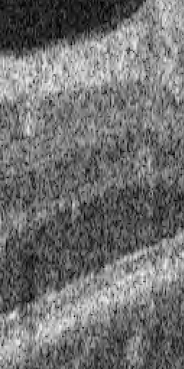
\includegraphics[width=0.18\linewidth]{figures/CirrusPatchExample.png}
	\caption{Example of a patch extracted from a Cirrus OCT volume used in Experiment 1.1. In this patch, while the background is noticeable due to its darker shade, the choroid is harder to be identified by an observer (or a model) due to the lack of context.}
	\label{fig:CirrusPatchExample}
\end{figure}

In Figure \ref{fig:Experiment11Segmentation} it is shown a segmentation performed by the model trained in Run 1 (see Table \ref{tab:Experiment1.1Results}). In this figure it becomes evident that the model learned which areas can be segmented inside the retina, but does not understand how the handle the regions further away. For example, in the area significantly above the retina the background is labeled as SRF. However, the background region closer to the retina is not so frequently labeled as any fluid, since it appears in the patches input to the model. The same problem occurs with the oversegmentation of PED in the choroid region, which does not appear in the input patches significantly.
\par
Oversegmentation beyond the retinal bounds is not exclusive to the Cirrus volumes, as it also appears in the OCT scans from other vendors. This suggests that the issue is primarily due to the small patch size rather than the smaller retinal area captured in Cirrus patches, despite this amplifying the problem. 
\par
In the same figure, it is seen that the model has not learned the anatomical relationships between fluids, since it segmented IRF and PED close to each other. This occurs because the model has not learned the relationship between the retinal landmarks and the fluid types due to the small sized inputs.

\begin{figure}[!ht]
	\centering
	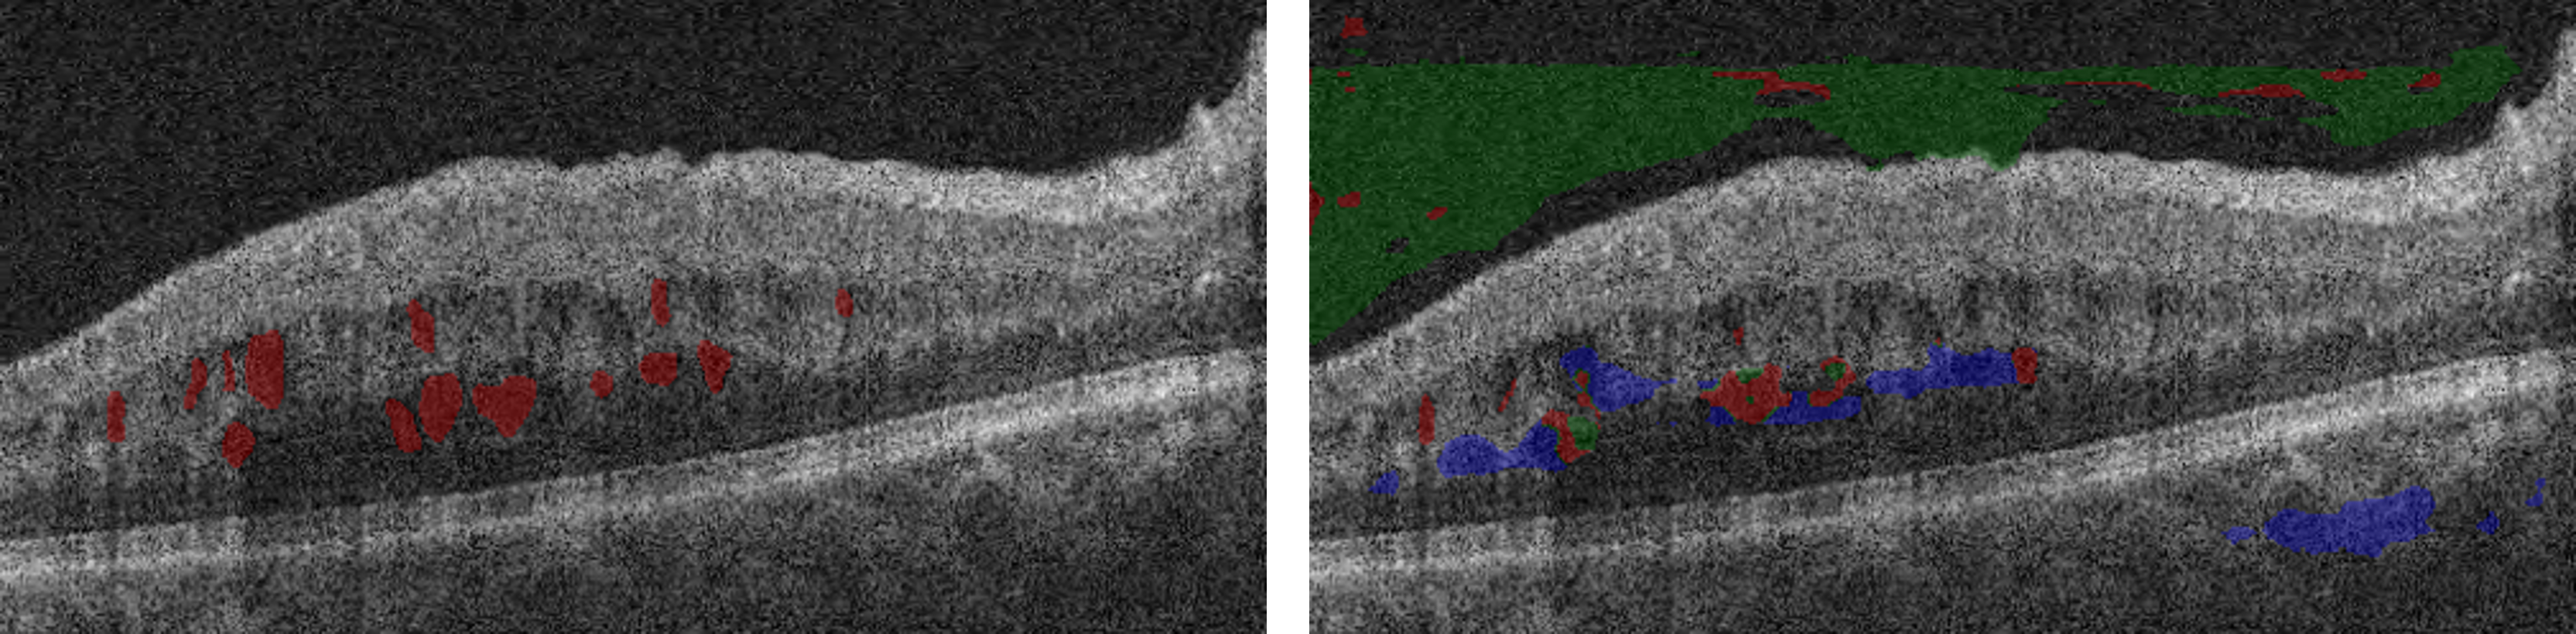
\includegraphics[width=1.0\linewidth]{figures/Experiment11Segmentation.png}
	\caption{Example of a poor segmentation made by the model trained in Run 1 (right). In the left, the GT mask for the same image is shown.}
	\label{fig:Experiment11Segmentation}
\end{figure}

\subsubsection{Experiment 1.2}

The resulting Dice coefficient values obtained in Experiment 1.2, where patches of shape 496 $\times$ 512 were used, are shown in Table \ref{tab:Experiment1.2Results}.

\begin{table*}[!ht]
	\caption{Dice scores for every vendor and fluid for the runs done in Experiment 1.2.}
	\centering
	\resizebox{\textwidth}{!}{\begin{tabular}{|c|c|ccc|ccc|ccc|c|c|c|c|}
		\hline
		% Headers
		\multirow{2}{*}{\textbf{Runs}} & 
		\multirow{2}{*}{\textbf{VF}} & 
		\multicolumn{3}{c|}{\textbf{Cirrus}} & 
		\multicolumn{3}{c|}{\textbf{Spectralis}} & 
		\multicolumn{3}{c|}{\textbf{Topcon}} & 
		\multicolumn{1}{c|}{\multirow{2}{*}{\textbf{IRF}}} & 
		\multirow{2}{*}{\textbf{SRF}} & 
		\multirow{2}{*}{\textbf{PED}} & 
		\multirow{2}{*}{\textbf{Fluid}} \\ \cline{3-11} & &
		\multicolumn{1}{c}{\textbf{IRF}} & 
		\multicolumn{1}{c}{\textbf{SRF}} & 
		\textbf{\textbf{PED}} & 
		\multicolumn{1}{c}{\textbf{IRF}} & 
		\multicolumn{1}{c}{\textbf{SRF}} & 
		\textbf{PED} & 
		\textbf{IRF} & 
		\textbf{SRF} & 
		\textbf{PED} & 
		\multicolumn{1}{c|}{} & & & \\ 
			
		\hline
		
		\textbf{Run 9} & 2 & \multicolumn{1}{c|}{0.291} & \multicolumn{1}{c|}{0.450} & 0.281 & \multicolumn{1}{c|}{0.472} & \multicolumn{1}{c|}{0.638} & 0.394 & \multicolumn{1}{c|}{0.505} & \multicolumn{1}{c|}{0.647} & 0.573 & 0.396 & 0.551 & 0.400 & 0.393 \\

		
		\textbf{Run 10} & 3 & \multicolumn{1}{c|}{\textbf{0.586}} & \multicolumn{1}{c|}{\textbf{0.619}} & \textbf{0.727} & \multicolumn{1}{c|}{0.482} & \multicolumn{1}{c|}{\textbf{0.780}} & \textbf{0.698} & \multicolumn{1}{c|}{\textbf{0.749}} & \multicolumn{1}{c|}{\textbf{0.793}} & \textbf{0.788} & \textbf{0.627} & \textbf{0.711} & \textbf{0.744} & \textbf{0.667} \\

		
		\textbf{Run 11} & 4 & \multicolumn{1}{c|}{0.281} & \multicolumn{1}{c|}{0.453} & 0.415 & \multicolumn{1}{c|}{0.429} & \multicolumn{1}{c|}{0.503} & 0.322 & \multicolumn{1}{c|}{0.228} & \multicolumn{1}{c|}{0.532} & 0.324 & 0.278 & 0.494 & 0.363 & 0.296 \\
		
		\textbf{Run 12} & 0 & \multicolumn{1}{c|}{0.242} & \multicolumn{1}{c|}{0.334} & 0.336 & \multicolumn{1}{c|}{\textbf{0.551}} & \multicolumn{1}{c|}{0.564} & 0.423 & \multicolumn{1}{c|}{0.321} & \multicolumn{1}{c|}{0.643} & 0.407 & 0.325 & 0.488 & 0.377 & 0.339 \\
		
		\hline
		
		\textbf{Set 3} & - & \multicolumn{1}{c|}{0.35} & \multicolumn{1}{c|}{0.46} & 0.44 & \multicolumn{1}{c|}{0.48} & \multicolumn{1}{c|}{0.62} & 0.46 & \multicolumn{1}{c|}{0.45} & \multicolumn{1}{c|}{0.65} & 0.52 & 0.41 & 0.56 & 0.47 & 0.42 \\
		
		\hline
					
	\end{tabular}}
	\label{tab:Experiment1.2Results}
\end{table*}

The information resumed in this table allows the comparison between the performance in models that used smaller patches in Experiment 1.1 with those that used larger patches in this Experiment.
\par
By comparing the ``Set'' rows, it becomes evident an overall increase in performance when using larger patches. In fact, it is observed an increase in almost all the mean values when compared to the best performing set in Experiment 1.1. This increase is larger than one decimal point in some columns, and the largest improvements occur in the volumes obtained using the Cirrus device and when segmenting SRF or PED.
\par
The improvement in performance in Cirrus devices can be explained with the more contextual information given. In Experiment 1.1, the Cirrus patches input to the model were not big enough for the network to capture and understand the retinal borders or the relationship between them and the fluids, thus leading to oversegmentation beyond the retina, as explained. In Experiment 1.2, as the same patch covers the retinal layer and the background simultaneously, the model has learned to not segment beyond the retina. In Figure \ref{fig:BigPatchesSegmentationCirrus}, the B-scan shown in Figure \ref{fig:Experiment11Segmentation}, is segmented by the model trained in Run 9 and it is possible to see that the labeling of the background as fluid is no longer happening.
\par 
This also partially justifies the significant improvement in the SRF and PED Dice coefficient. By providing inputs with enough context, the model is no longer segmenting these fluids outside the retina. However, in Figure \ref{fig:BigPatchesSegmentationCirrus} it is also seen that the model is no longer confusing the fluids in the retina, as it no longer segments the PED close to the IRF. This further justifies that the model is learning the anatomical references associated with PED, as confirmed in Figure \ref{fig:BigPatchesSegmentationTopcon}.
\par
Lastly, it is important to note that the IRF did not improve as much as the other fluids. This happens because the input patches in Experiment 1.1 where extracted mainly from the retina, providing all the anatomical context needed for the IRF segmentation.
\par
In Figure \ref{fig:BigPatchesSegmentationTopcon}, it is seen that the model confuses the choroid with the retina, as it labels parts of that region as IRF and PED. The likely cause for this confusion is that the input patches are often cropped in the middle of the retinal layer (as illustrated in Figure \ref{fig:BigPatchExtraction}), which leads to the model not understanding the position of the choroid relative to the retina. This inaccurate IRF and PED segmentation is probably based on the visual resemblance between the structures seen in the choroid and the fluid pockets in the retina. This indicates that the model does not know the location of the choroid.

\begin{figure}[!ht]
	\centering
	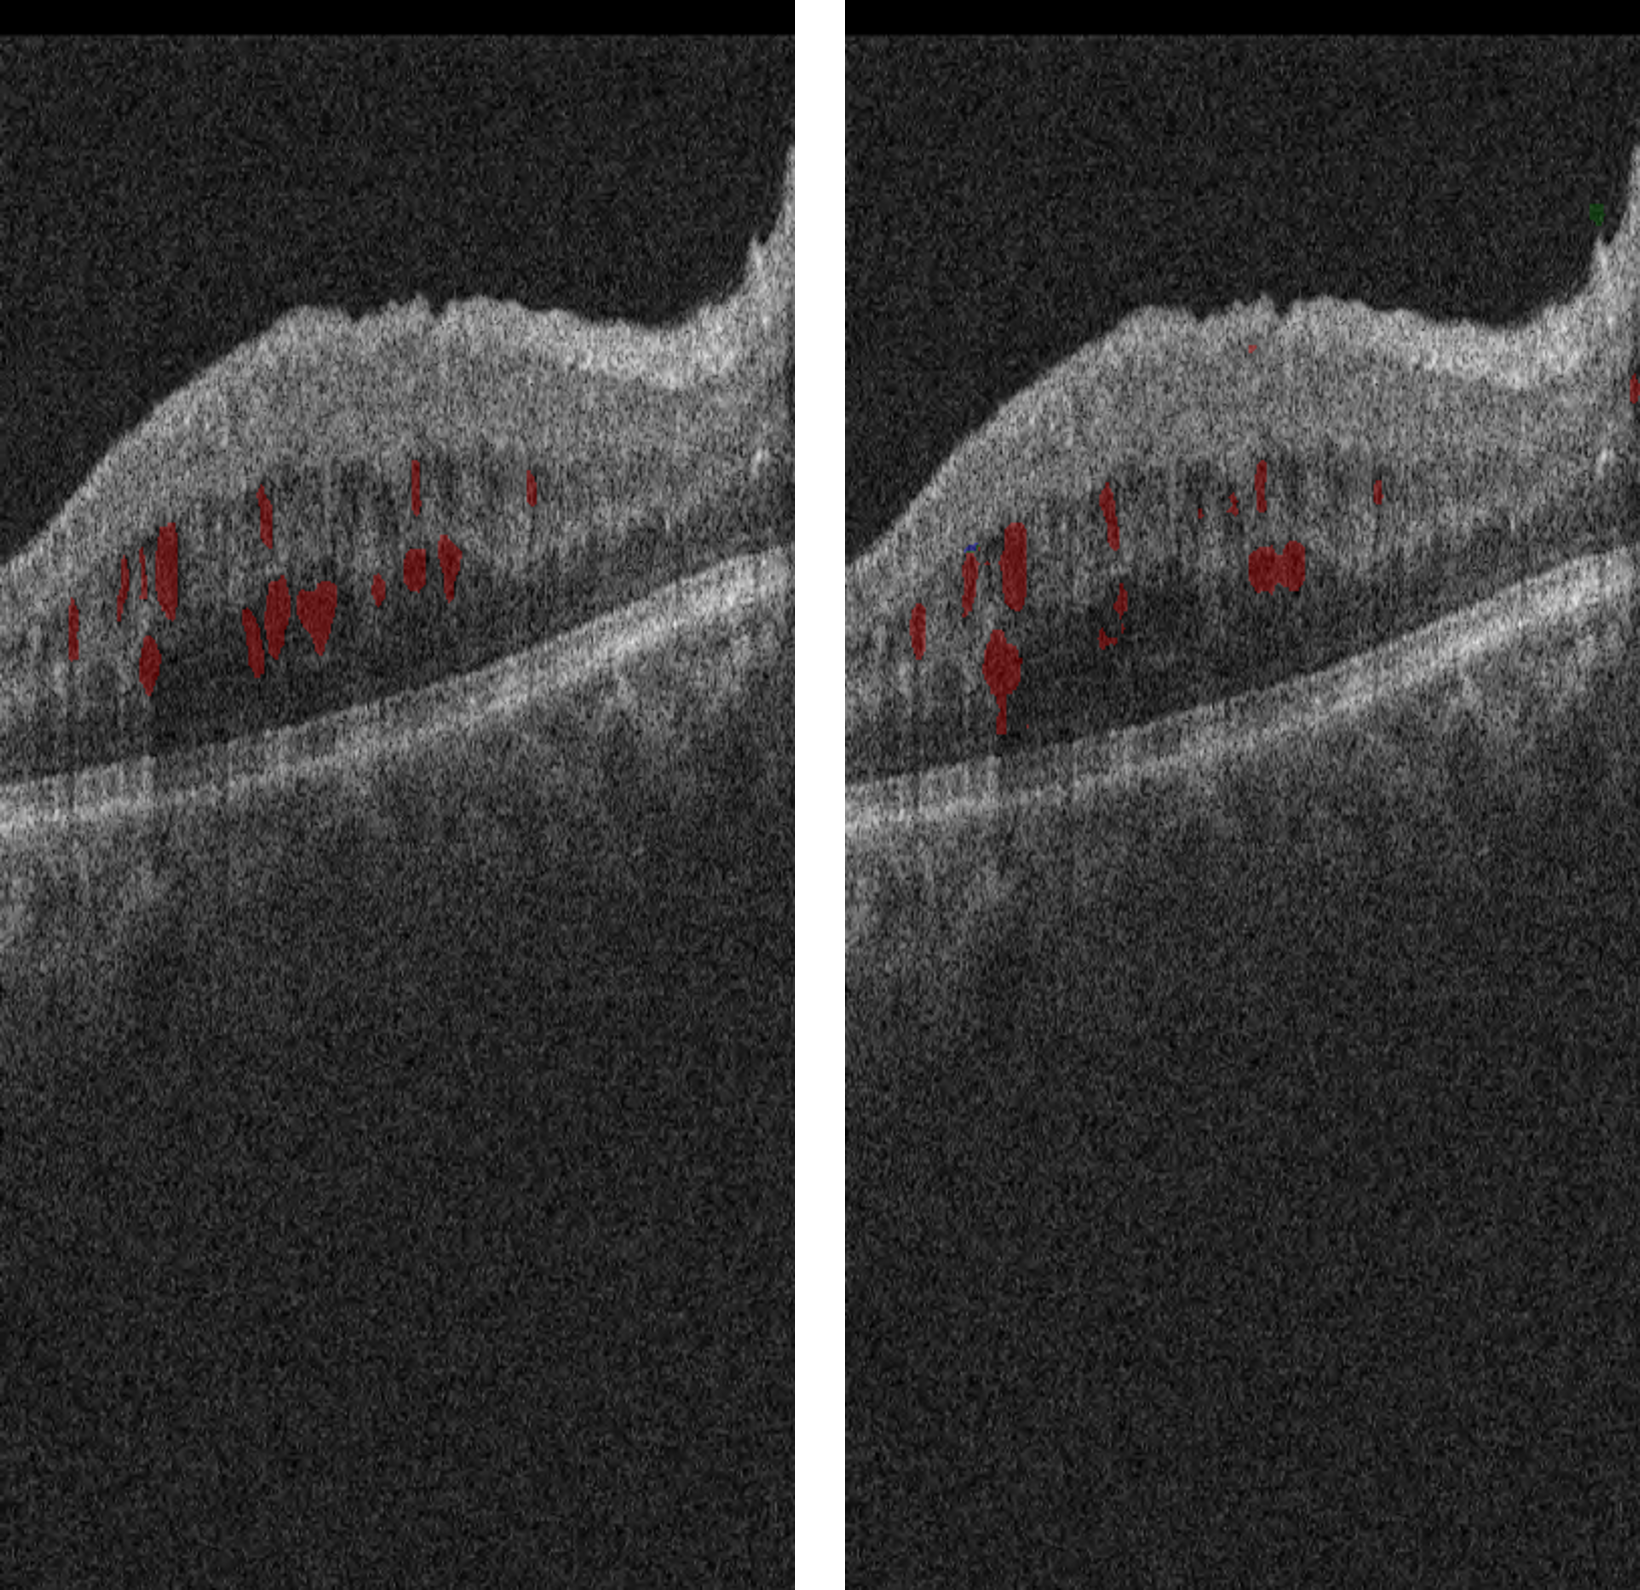
\includegraphics[width=0.5\linewidth]{figures/BigPatchSegmentationCirrus.png}
	\caption{Example of the segmentation done by the model trained in Run 9 (right) and its respective GT mask (left). The B-scan segmented is the same as in Figure \ref{fig:Experiment11Segmentation}.}
	\label{fig:BigPatchesSegmentationCirrus}
\end{figure}

\begin{figure}[!ht]
	\centering
	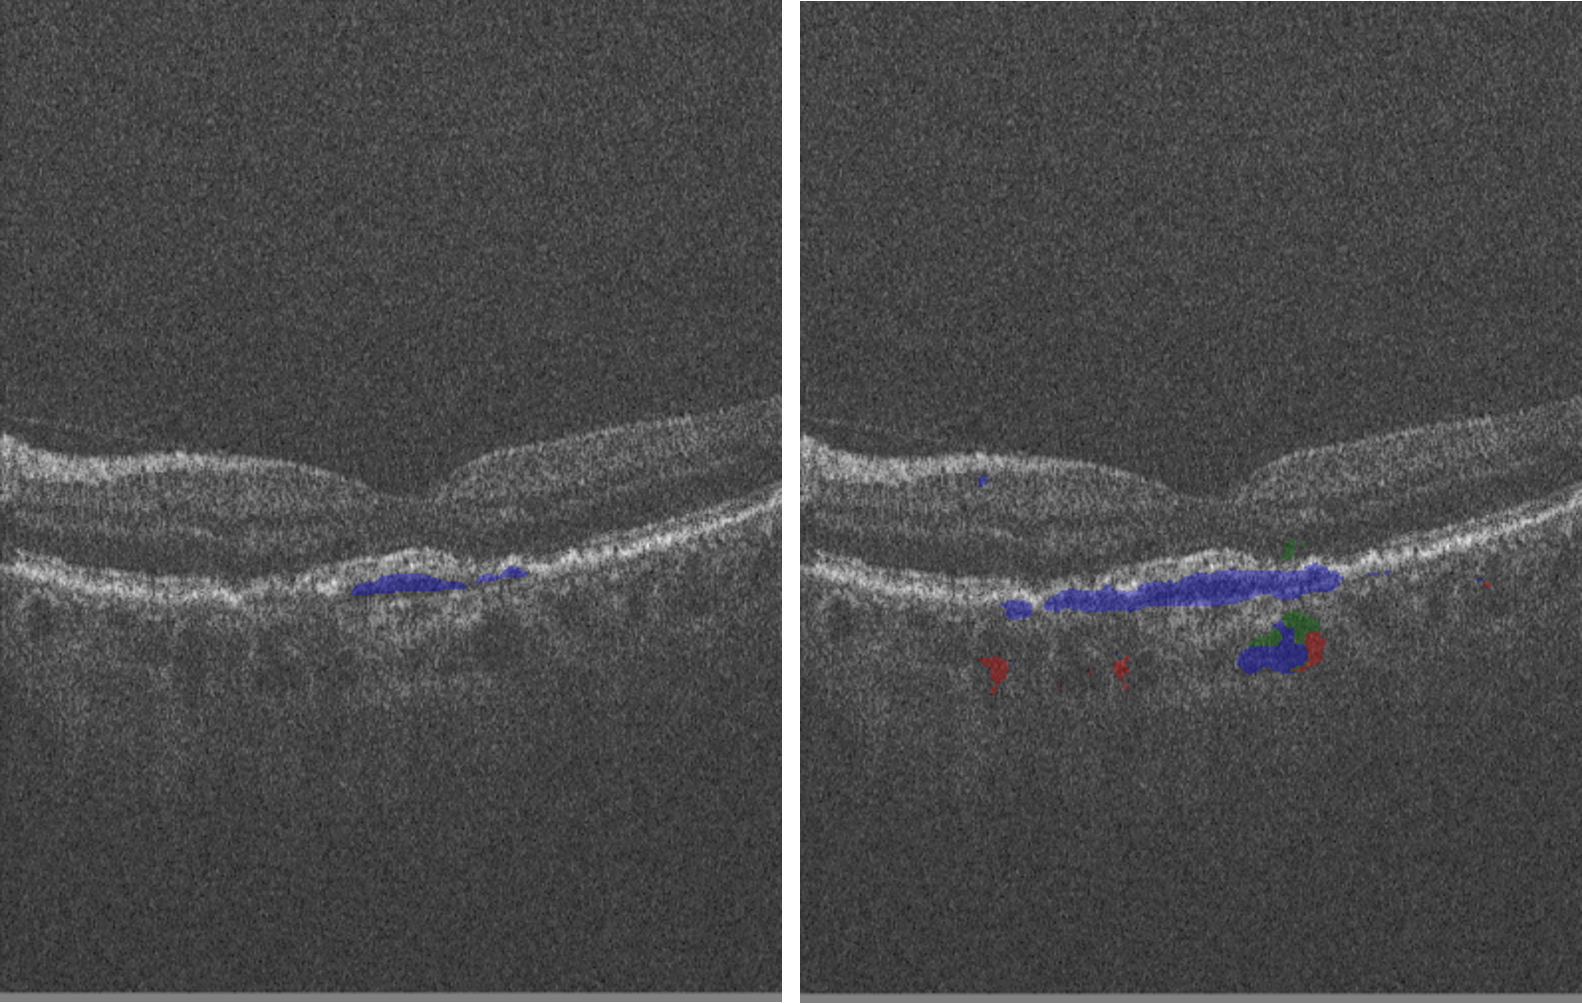
\includegraphics[width=0.6\linewidth]{figures/BigPatchSegmentationTopcon.png}
	\caption{Example of the segmentation done by the model trained in Run 12 (right) and its respective GT mask (left). It is noticeable that the model confuses the choroid with the retina, as segmentation of IRF and PED is performed in the choroid.}
	\label{fig:BigPatchesSegmentationTopcon}
\end{figure}

\subsubsection{Experiment 1.3}
Experiment 1.3 contains all the runs that were performed using vertical patches extracted from resized B-scans as input of the multi-class segmentation U-Net. In the first two sets, shown in Table \ref{tab:Experiment1.3FourPatches}, the models were trained using four vertical patches, obtained as explained in the \ref{Methods} Methods chapter. In this table, the ``Set 4'' is composed of runs that were trained on 100 epochs, while the runs in ``Set 5'' were trained on up to 200 epochs with a 100 epoch patience.

\begin{table*}[!ht]
	\caption{Dice scores for every vendor and fluid for the runs done using four vertical patches extracted from each B-scan. In ``Set 4'', the models were trained in 100 epochs, while in ``Set 5'' the models were trained on up to 200 epochs with a 100 epoch patience. The transformations applied in these sets were the same: horizontal flipping and a maximum rotation of $10^{\circ}$.}
	\centering
	\resizebox{\textwidth}{!}{\begin{tabular}{|c|c|ccc|ccc|ccc|c|c|c|c|}
		\hline
		% Headers
		\multirow{2}{*}{\textbf{Runs}} & 
		\multirow{2}{*}{\textbf{VF}} & 
		\multicolumn{3}{c|}{\textbf{Cirrus}} & 
		\multicolumn{3}{c|}{\textbf{Spectralis}} & 
		\multicolumn{3}{c|}{\textbf{Topcon}} & 
		\multicolumn{1}{c|}{\multirow{2}{*}{\textbf{IRF}}} & 
		\multirow{2}{*}{\textbf{SRF}} & 
		\multirow{2}{*}{\textbf{PED}} & 
		\multirow{2}{*}{\textbf{Fluid}} \\ \cline{3-11} & &
		\multicolumn{1}{c}{\textbf{IRF}} & 
		\multicolumn{1}{c}{\textbf{SRF}} & 
		\textbf{\textbf{PED}} & 
		\multicolumn{1}{c}{\textbf{IRF}} & 
		\multicolumn{1}{c}{\textbf{SRF}} & 
		\textbf{PED} & 
		\textbf{IRF} & 
		\textbf{SRF} & 
		\textbf{PED} & 
		\multicolumn{1}{c|}{} & & & \\ 
			
		\hline
		
		\textbf{Run 13} & 2 & \multicolumn{1}{c|}{0.411} & \multicolumn{1}{c|}{0.665} & 0.498 & \multicolumn{1}{c|}{0.654} & \multicolumn{1}{c|}{0.735} & 0.611 & \multicolumn{1}{c|}{0.731} & \multicolumn{1}{c|}{0.743} & 0.519 & 0.563 & 0.704 & 0.526 & 0.581 \\

		\textbf{Run 14} & 3 & \multicolumn{1}{c|}{0.390} & \multicolumn{1}{c|}{0.520} & 0.217 & \multicolumn{1}{c|}{0.403} & \multicolumn{1}{c|}{0.564} & 0.429 & \multicolumn{1}{c|}{0.378} & \multicolumn{1}{c|}{0.754} & 0.477 & 0.388 & 0.614 & 0.350 & 0.386 \\
		
		\textbf{Run 15} & 4 & \multicolumn{1}{c|}{0.792} & \multicolumn{1}{c|}{\textbf{0.846}} & \textbf{0.883} & \multicolumn{1}{c|}{0.732} & \multicolumn{1}{c|}{\textbf{0.901}} & 0.733 & \multicolumn{1}{c|}{0.615} & \multicolumn{1}{c|}{0.758} & 0.656 & 0.707 & 0.815 & 0.765 & 0.652 \\
		
		\textbf{Run 16} & 0 & \multicolumn{1}{c|}{\textbf{0.810}} & \multicolumn{1}{c|}{0.834} & 0.715 & \multicolumn{1}{c|}{0.779} & \multicolumn{1}{c|}{0.857} & 0.753 & \multicolumn{1}{c|}{0.783} & \multicolumn{1}{c|}{\textbf{0.924}} & \textbf{0.882} & \textbf{0.795} & \textbf{0.871} & \textbf{0.783} & \textbf{0.709} \\
		
		\hline
		
		\textbf{Set 4} & - & \multicolumn{1}{c|}{\textbf{0.60}} & \multicolumn{1}{c|}{\textbf{0.72}} & 0.58 & \multicolumn{1}{c|}{0.64} & \multicolumn{1}{c|}{\textbf{0.76}} & 0.63 & \multicolumn{1}{c|}{0.63} & \multicolumn{1}{c|}{\textbf{0.79}} & 0.63 & 0.61 & \textbf{0.75} & 0.61 & 0.58 \\
		
		\hline
		\hline
		
		\textbf{Run 17} & 2 & \multicolumn{1}{c|}{0.522} & \multicolumn{1}{c|}{0.784} & 0.703 & \multicolumn{1}{c|}{\textbf{0.805}} & \multicolumn{1}{c|}{0.765} & \textbf{0.865} & \multicolumn{1}{c|}{\textbf{0.828}} & \multicolumn{1}{c|}{0.879} & 0.835 & 0.677 & 0.813 & 0.777 & 0.684 \\
	
		\textbf{Run 18} & 3 & \multicolumn{1}{c|}{0.509} & \multicolumn{1}{c|}{0.654} & 0.598 & \multicolumn{1}{c|}{0.590} & \multicolumn{1}{c|}{0.806} & 0.755 & \multicolumn{1}{c|}{0.777} & \multicolumn{1}{c|}{0.787} & 0.792 & 0.621 & 0.729 & 0.697 & 0.622 \\
					
		\textbf{Run 19} & 4 & \multicolumn{1}{c|}{0.377} & \multicolumn{1}{c|}{0.387} & 0.398 & \multicolumn{1}{c|}{0.478} & \multicolumn{1}{c|}{0.624} & 0.398 & \multicolumn{1}{c|}{0.483} & \multicolumn{1}{c|}{0.729} & 0.448 & 0.436 & 0.567 & 0.420 & 0.399 \\
		
		\textbf{Run 20} & 0 & \multicolumn{1}{c|}{0.753} & \multicolumn{1}{c|}{0.697} & 0.696 & \multicolumn{1}{c|}{0.779} & \multicolumn{1}{c|}{0.844} & 0.783 & \multicolumn{1}{c|}{0.691} & \multicolumn{1}{c|}{0.720} & 0.671 & 0.735 & 0.731 & 0.702 & 0.637 \\
		
		\hline
		
		\textbf{Set 5} & - & \multicolumn{1}{c|}{0.54} & \multicolumn{1}{c|}{0.63} & \textbf{0.60} & \multicolumn{1}{c|}{\textbf{0.66}} & \multicolumn{1}{c|}{0.76} & \textbf{0.70} & \multicolumn{1}{c|}{\textbf{0.69}} & \multicolumn{1}{c|}{0.78} & \textbf{0.69} & \textbf{0.62} & 0.71 & \textbf{0.65} & \textbf{0.59} \\
		
		\hline
			
	\end{tabular}}
	\label{tab:Experiment1.3FourPatches}
\end{table*}

The results of the sets shown in Table \ref{tab:Experiment1.3FourPatches} can be compared within each other and to the results obtained in the sets of previous experiments. 
\par
When comparing the results between sets, it is noticeable that the runs with the best scores are mostly located in the ``Set'' that trained less epochs. For, the model validated on fold 4 (Run 15) sees a significant decrease in performance when trained for 100 more epochs (Run 19). When looking at the models validation loss per epoch, the lowest value is attained commonly before the 100 epochs. Since the model that is saved in each run is the model that attains the lowest loss on validation data, this means that the models trained in 100 or 200 epochs should perform equally, as long as the lowest validation loss occurred prior to the 100 epoch mark.
\par
However, looking at Figure \ref{fig:TrainingValidationLosses}, where the training and validation loss curves for the Run 13 and Run 17 are shown, similar trends and behavior is seen in both models. This does not reflect to similar performances in the same validation data, as shown in Table \ref{tab:Experiment1.3FourPatches}. In fact, a substantial increment is seen in Run 17.
\par
To justify this behavior, it is important to remind that the training of a neural network has some randomness associated with it. One aspect that affects the model performance despite using the same data and architecture is the weight initialization. The random initialization of weights affects the trajectory of gradient descent, resulting in different convergences for different runs. Another factor that affects the model learning is the data that composes each batch. The images that form a batch are randomly fetch from the available input images. This create batches with different distributions of characteristics, affecting the model's view of the data. Data augmentation, which randomly selects images to apply the transformations as they are fetch, also influences the model performance. Lastly, there are other factors that have a much smaller impact such as the optimizer behavior and non-deterministic operations at the GPU level \parencite{Akesson2024, Altarabichi2024}. 
\par
In Appendix \ref{ap1:SegmentationUNetVariability}, Table \ref{tab:SegmentationUNetVariability} shows the results for multiple models that were trained on the same conditions, aiming to give an insight on how the randomness associated with the U-Net affects the models performances. Five models were validated on fold 2, while nine models were validated in fold 3. The results obtained corroborate the differences seen in Table \ref{tab:Experiment1.3FourPatches}, where models trained on the same conditions for more epochs can obtain significantly worse Dice scores in validation.

\begin{figure}[!ht]
	\centering
	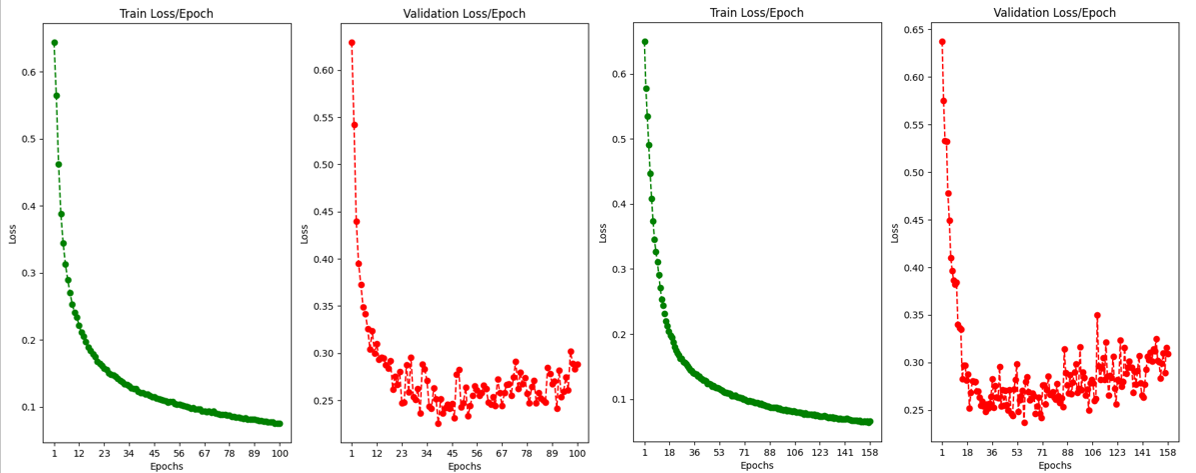
\includegraphics[width=1.0\linewidth]{figures/TrainingValidationLosses.png}
	\caption{Training and validation losses in Run 13 (left) and Run 17 (right). Despite reaching the validation loss minimum in a similar number of epochs and having comparable training and validation loss curves, the performance is really different in Table \ref{tab:Experiment1.3FourPatches}.}
	\label{fig:TrainingValidationLosses}
\end{figure}

Despite the differences in the results shown in Table \ref{tab:Experiment1.3FourPatches}, both sets attained better performances than the best results in the previous experiments. The improvements were significant, registering increases above 0.2 in some metrics when compared with the results in Experiment 1.3. Every vendor and every fluid seen a considerable increase of performance.
\par
This overall increment can be attributed to two changes: training on vertical patches and resizing the images. By training the models on vertical patches, the model can focus on the finer details within each region. This is important because the retinal fluid segmentation relies heavily on the retina's characteristics, a region that occupies a small portion of the image. Despite the input being smaller than in Experiment 1.3, the patches could still capture the transitions between the retina and the choroid or background. Since the input size is smaller, less storage it occupies in memory, therefore allowing an increase in the batch size, that translates to a faster and more stable convergence. Meanwhile, the image's resizing makes the inputs more homogeneous across different vendors. This results in the same structures being represented with consistent shapes and sizes across the B-scans from different vendors, resulting in a significantly simpler learning process.
\par
It was seen in Figure \ref{fig:BigPatchesSegmentationTopcon} that the model predicted fluid masks in the choroid region. In Figure \ref{fig:VerticalPatchesSegmentationTopcon}, it is seen that the models trained on vertical patches no longer predict fluid in the choroid region, despite inferring on the same B-scan. This means that, by feeding vertical patches to the model, it learns to not segment below the retina, in the choroid. This was not previously understood by the model when big patches were input, since these would frequently not capture both the retinal layer and the choroid in the same patch, restraining the model from learning the relative position of the choroid and its relationship with the fluid prediction.

\begin{figure}[!ht]
	\centering
	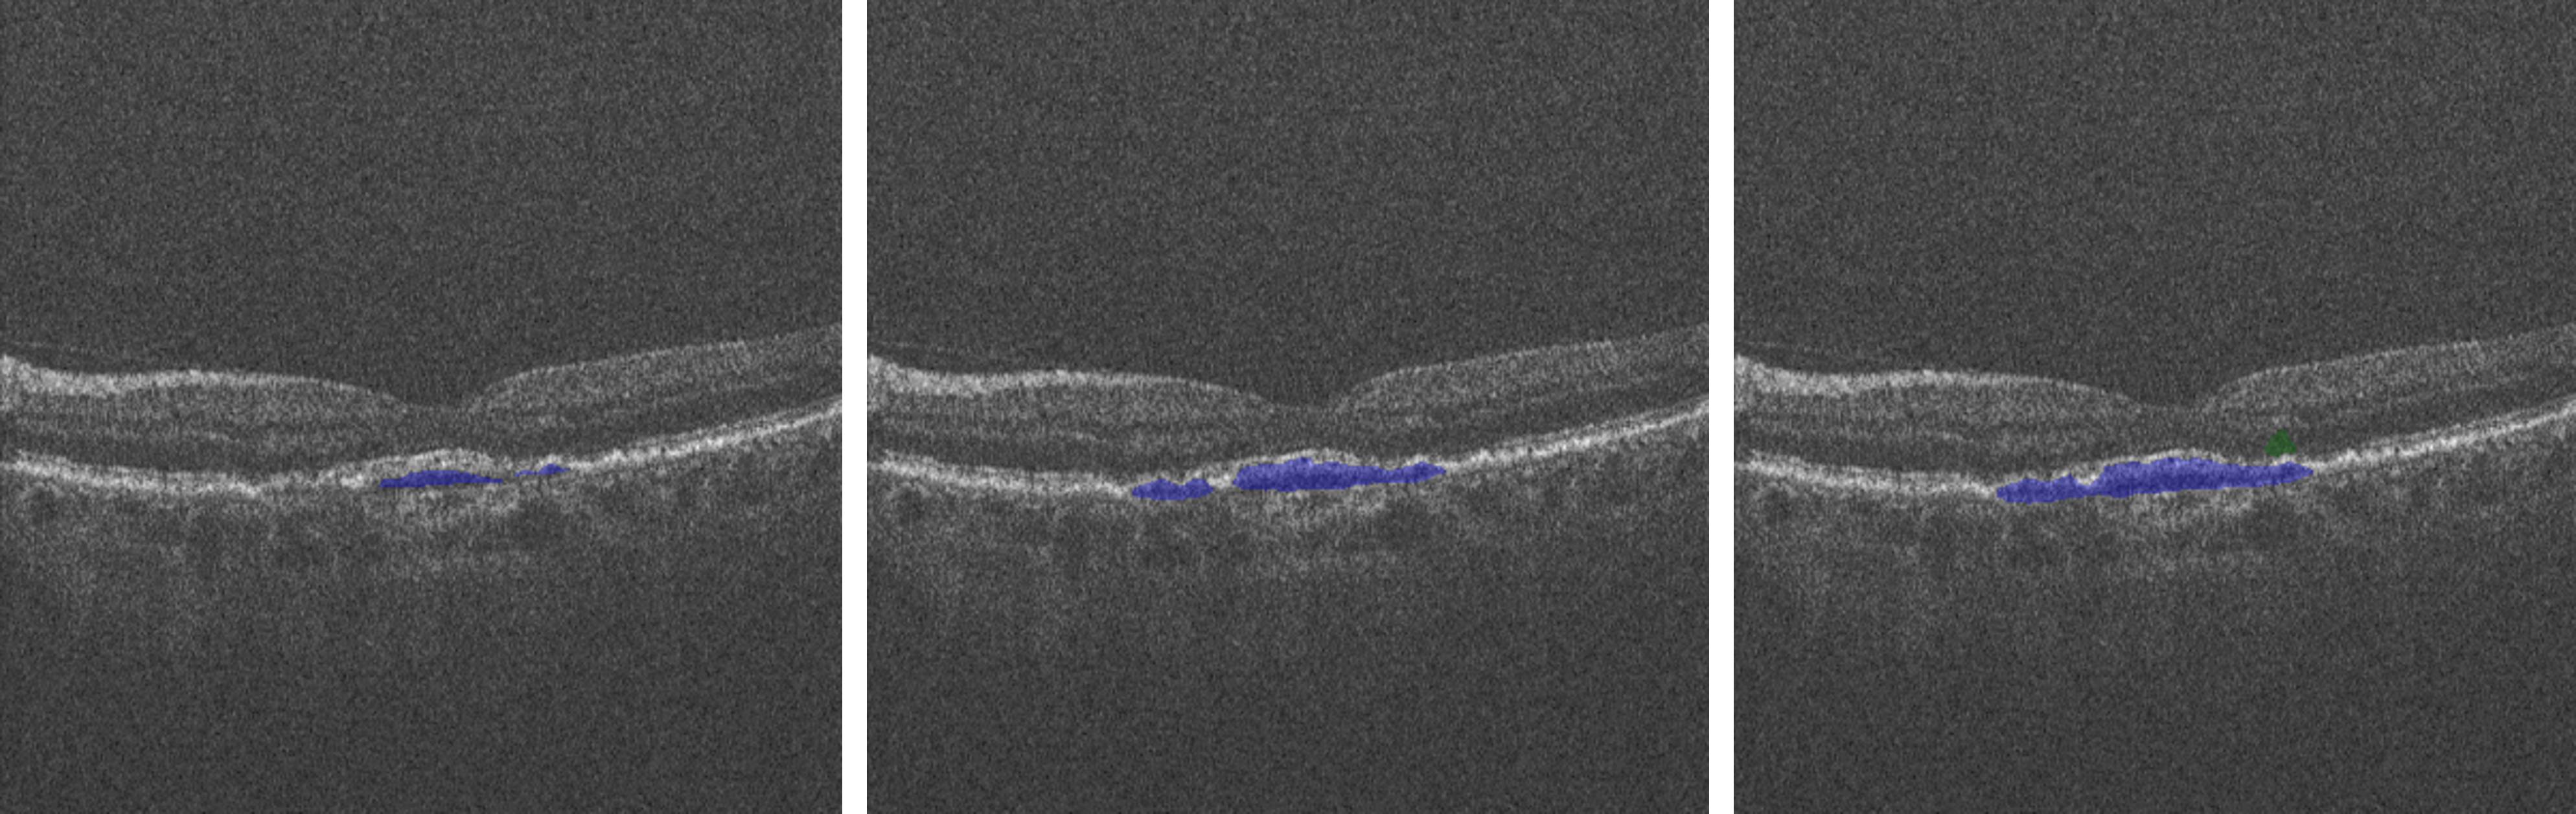
\includegraphics[width=1.0\linewidth]{figures/VerticalPatchesSegmentationTopcon.png}
	\caption{Predicted masks by the models trained on Run 16 (middle) and Run 20 (right) and their respective GT (left).}
	\label{fig:VerticalPatchesSegmentationTopcon}
\end{figure}

Afterwards, the use of seven and thirteen patches extracted from each B-scan was tested and the results are shown in Table \ref{tab:Experiment1.3SevenVsThirteenPatches}. Two models were trained for each number of patches extracted, one validated on fold 2 and another validated on fold 3. The models were trained on 200 maximum epochs, with a 25 epoch patience applied after the first 100 epochs.

\begin{table*}[!ht]
	\caption{Dice scores for every vendor and fluid for the runs done using seven (Runs 21 and 22) and thirteen (Runs 23 and 24) vertical patches extracted from each B-scan. Only two folds were used in order to understand the viability of using these numbers of patches.}
	\centering
	\resizebox{\textwidth}{!}{\begin{tabular}{|c|c|ccc|ccc|ccc|c|c|c|c|}
		\hline
		% Headers
		\multirow{2}{*}{\textbf{Runs}} & 
		\multirow{2}{*}{\textbf{VF}} & 
		\multicolumn{3}{c|}{\textbf{Cirrus}} & 
		\multicolumn{3}{c|}{\textbf{Spectralis}} & 
		\multicolumn{3}{c|}{\textbf{Topcon}} & 
		\multicolumn{1}{c|}{\multirow{2}{*}{\textbf{IRF}}} & 
		\multirow{2}{*}{\textbf{SRF}} & 
		\multirow{2}{*}{\textbf{PED}} & 
		\multirow{2}{*}{\textbf{Fluid}} \\ \cline{3-11} & &
		\multicolumn{1}{c}{\textbf{IRF}} & 
		\multicolumn{1}{c}{\textbf{SRF}} & 
		\textbf{\textbf{PED}} & 
		\multicolumn{1}{c}{\textbf{IRF}} & 
		\multicolumn{1}{c}{\textbf{SRF}} & 
		\textbf{PED} & 
		\textbf{IRF} & 
		\textbf{SRF} & 
		\textbf{PED} & 
		\multicolumn{1}{c|}{} & & & \\ 
			
		\hline
		
		\textbf{Run 21} & 2 & \multicolumn{1}{c|}{0.556} & \multicolumn{1}{c|}{0.837} & 0.672 & \multicolumn{1}{c|}{\textbf{0.761}} & \multicolumn{1}{c|}{\textbf{0.853}} & \textbf{0.848} & \multicolumn{1}{c|}{\textbf{0.829}} & \multicolumn{1}{c|}{0.908} & \textbf{0.858} & 0.685 & \textbf{0.864} & 0.767 & \textbf{0.681} \\
		
		\textbf{Run 22} & 3 & \multicolumn{1}{c|}{\textbf{0.734}} & \multicolumn{1}{c|}{\textbf{0.855}} & 0.836 & \multicolumn{1}{c|}{0.636} & \multicolumn{1}{c|}{0.846} & 0.689 & \multicolumn{1}{c|}{0.686} & \multicolumn{1}{c|}{0.781} & 0.731 & \textbf{0.700} & 0.822 & \textbf{0.771} & 0.672 \\
		
		\hline
		\hline
		
		\textbf{Run 23} & 2 & \multicolumn{1}{c|}{0.500} & \multicolumn{1}{c|}{0.762} & 0.635 & \multicolumn{1}{c|}{0.672} & \multicolumn{1}{c|}{0.790} & 0.773 & \multicolumn{1}{c|}{0.819} & \multicolumn{1}{c|}{\textbf{0.936}} & 0.805 & 0.639 & 0.826 & 0.718 & 0.637 \\
		
		\textbf{Run 24} & 3 & \multicolumn{1}{c|}{0.612} & \multicolumn{1}{c|}{0.648} & \textbf{0.882} & \multicolumn{1}{c|}{0.455} & \multicolumn{1}{c|}{0.636} & 0.548 & \multicolumn{1}{c|}{0.499} & \multicolumn{1}{c|}{0.593} & 0.668 & 0.542 & 0.622 & 0.745 & 0.536 \\
		
		\hline
			
	\end{tabular}}
	\label{tab:Experiment1.3SevenVsThirteenPatches}
\end{table*}

Training the models on more patches per B-scan, significantly increases the quantity of data that is seen by the model during an epoch. Therefore, each epoch takes much longer to complete, requiring more computation power, leading to often bottlenecks. However, since the model sees many more patches per epoch, the model reaches the validation loss minimum much earlier than in the models trained with four patches. In Figure , it is possible to see a comparison between the training and validation losses of the models validated on fold 2, using four, seven, and thirteen vertical patches per B-scan.

\begin{figure}[!ht]
	\centering
	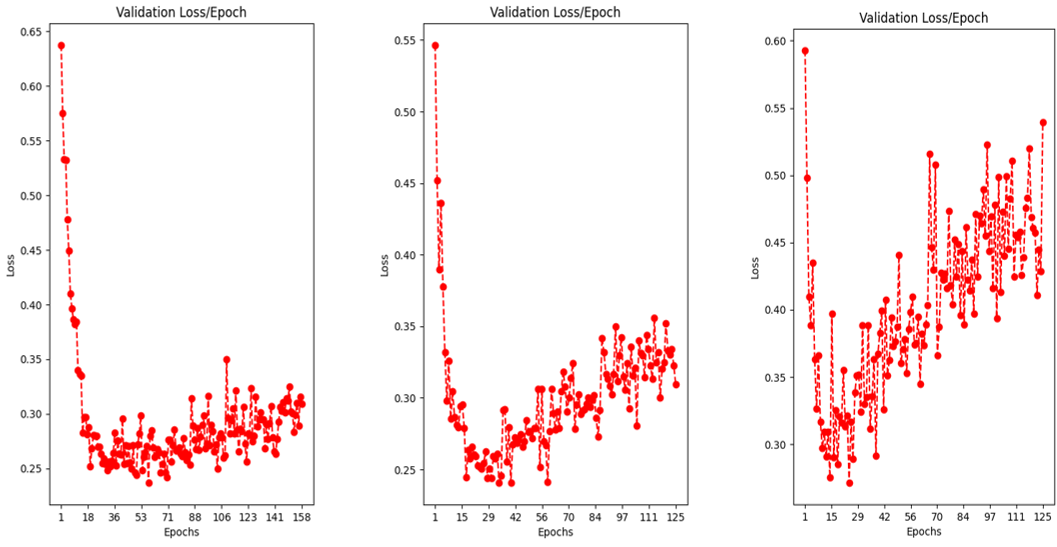
\includegraphics[width=1.0\linewidth]{figures/ValidationLossesFourSevenThirteenPatches.png}
	\caption{Training and validation losses for models validated on fold 2. The curves on the left are from the model trained on Run 13 with four patches, while the middle curves are from the model trained on Run 21, with seven patches. The curves on the right are from the model trained on Run 23, with thirteen patches.}
	\label{fig:ValidationLossesFourSevenThirteenPatches}
\end{figure}

\begin{table*}[!ht]
	\caption{Dice scores for every vendor and fluid using seven vertical patches. The only transformation performed in these runs was horizontal flipping, without rotation.}
	\centering
	\resizebox{\textwidth}{!}{\begin{tabular}{|c|c|ccc|ccc|ccc|c|c|c|c|}
			\hline
			% Headers
			\multirow{2}{*}{\textbf{Runs}} & 
			\multirow{2}{*}{\textbf{VF}} & 
			\multicolumn{3}{c|}{\textbf{Cirrus}} & 
			\multicolumn{3}{c|}{\textbf{Spectralis}} & 
			\multicolumn{3}{c|}{\textbf{Topcon}} & 
			\multicolumn{1}{c|}{\multirow{2}{*}{\textbf{IRF}}} & 
			\multirow{2}{*}{\textbf{SRF}} & 
			\multirow{2}{*}{\textbf{PED}} & 
			\multirow{2}{*}{\textbf{Fluid}} \\ \cline{3-11} & &
			\multicolumn{1}{c}{\textbf{IRF}} & 
			\multicolumn{1}{c}{\textbf{SRF}} & 
			\textbf{\textbf{PED}} & 
			\multicolumn{1}{c}{\textbf{IRF}} & 
			\multicolumn{1}{c}{\textbf{SRF}} & 
			\textbf{PED} & 
			\textbf{IRF} & 
			\textbf{SRF} & 
			\textbf{PED} & 
			\multicolumn{1}{c|}{} & & & \\ 
			
			\hline
			
			\textbf{Run 25} & 2 & \multicolumn{1}{c|}{0.406} & \multicolumn{1}{c|}{0.789} & 0.656 & \multicolumn{1}{c|}{0.595} & \multicolumn{1}{c|}{\textbf{0.805}} & \textbf{0.786} & \multicolumn{1}{c|}{0.762} & \multicolumn{1}{c|}{0.841} & 0.797 & 0.560 & 0.809 & 0.727 & 0.620 \\

			
			\textbf{Run 26} & 3 & \multicolumn{1}{c|}{0.589} & \multicolumn{1}{c|}{0.775} & 0.553 & \multicolumn{1}{c|}{0.586} & \multicolumn{1}{c|}{0.803} & 0.766 & \multicolumn{1}{c|}{0.769} & \multicolumn{1}{c|}{\textbf{0.827}} & 0.755 & 0.654 & 0.799 & 0.664 & 0.617 \\
			
			
			\textbf{Run 27} & 4 & \multicolumn{1}{c|}{\textbf{0.797}} & \multicolumn{1}{c|}{\textbf{0.845}} & \textbf{0.827} & \multicolumn{1}{c|}{\textbf{0.734}} & \multicolumn{1}{c|}{0.782} & 0.659 & \multicolumn{1}{c|}{0.533} & \multicolumn{1}{c|}{0.756} & 0.553 & 0.674 & 0.798 & 0.686 & 0.626 \\
			
			
			\textbf{Run 28} & 0 & \multicolumn{1}{c|}{0.677} & \multicolumn{1}{c|}{0.842} & 0.699 & \multicolumn{1}{c|}{0.681} & \multicolumn{1}{c|}{0.799} & 0.732 & \multicolumn{1}{c|}{\textbf{0.791}} & \multicolumn{1}{c|}{0.846} & \textbf{0.854} & \textbf{0.719} & \textbf{0.836} & \textbf{0.762} & \textbf{0.665} \\
			
			
			\hline
			
			\textbf{Set 6} & - & \multicolumn{1}{c|}{0.62} & \multicolumn{1}{c|}{0.81} & 0.68 & \multicolumn{1}{c|}{0.65} & \multicolumn{1}{c|}{0.80} & 0.74 & \multicolumn{1}{c|}{0.71} & \multicolumn{1}{c|}{0.82} & 0.74 & 0.65 & 0.81 & 0.71 & 0.63 \\
			
			\hline
			
	\end{tabular}}
	\label{tab:Experiment1.3SevenPatchesNoRotation}
\end{table*}

\begin{table*}[!ht]
	\caption{Dice scores for every vendor and fluid using seven vertical patches. In these runs, horizontal flipping and $5^{\circ}$ rotation were used, instead of the usual $10^{\circ}$.}
	\centering
	\resizebox{\textwidth}{!}{\begin{tabular}{|c|c|ccc|ccc|ccc|c|c|c|c|}
		\hline
		% Headers
		\multirow{2}{*}{\textbf{Runs}} & 
		\multirow{2}{*}{\textbf{VF}} & 
		\multicolumn{3}{c|}{\textbf{Cirrus}} & 
		\multicolumn{3}{c|}{\textbf{Spectralis}} & 
		\multicolumn{3}{c|}{\textbf{Topcon}} & 
		\multicolumn{1}{c|}{\multirow{2}{*}{\textbf{IRF}}} & 
		\multirow{2}{*}{\textbf{SRF}} & 
		\multirow{2}{*}{\textbf{PED}} & 
		\multirow{2}{*}{\textbf{Fluid}} \\ \cline{3-11} & &
		\multicolumn{1}{c}{\textbf{IRF}} & 
		\multicolumn{1}{c}{\textbf{SRF}} & 
		\textbf{\textbf{PED}} & 
		\multicolumn{1}{c}{\textbf{IRF}} & 
		\multicolumn{1}{c}{\textbf{SRF}} & 
		\textbf{PED} & 
		\textbf{IRF} & 
		\textbf{SRF} & 
		\textbf{PED} & 
		\multicolumn{1}{c|}{} & & & \\ 
		
		\hline
		
		\textbf{Run 29} & 2 & \multicolumn{1}{c|}{0.497} & \multicolumn{1}{c|}{0.783} & 0.609 & \multicolumn{1}{c|}{0.763} & \multicolumn{1}{c|}{0.851} & 0.822 & \multicolumn{1}{c|}{0.832} & \multicolumn{1}{c|}{\textbf{0.904}} & 0.799 & 0.658 & 0.836 & 0.712 & 0.666 \\
		
		\textbf{Run 30} & 3 & \multicolumn{1}{c|}{0.475} & \multicolumn{1}{c|}{0.747} & 0.613 & \multicolumn{1}{c|}{0.656} & \multicolumn{1}{c|}{0.846} & 0.757 & \multicolumn{1}{c|}{\textbf{0.856}} & \multicolumn{1}{c|}{0.869} & \textbf{0.835} & 0.646 & 0.809 & 0.720 & 0.646 \\
		
		\textbf{Run 31} & 4 & \multicolumn{1}{c|}{0.643} & \multicolumn{1}{c|}{0.709} & 0.747 & \multicolumn{1}{c|}{0.627} & \multicolumn{1}{c|}{0.800} & 0.635 & \multicolumn{1}{c|}{0.457} & \multicolumn{1}{c|}{0.599} & 0.529 & 0.560 & 0.673 & 0.638 & 0.523 \\
		
		\textbf{Run 32} & 0 & \multicolumn{1}{c|}{\textbf{0.794}} & \multicolumn{1}{c|}{\textbf{0.878}} & \textbf{0.770} & \multicolumn{1}{c|}{\textbf{0.807}} & \multicolumn{1}{c|}{\textbf{0.902}} & \textbf{0.862} & \multicolumn{1}{c|}{0.796} & \multicolumn{1}{c|}{0.842} & 0.830 & \textbf{0.797} & \textbf{0.869} & \textbf{0.808} & \textbf{0.698} \\
		
		\hline
		
		\textbf{Set 7} & - & \multicolumn{1}{c|}{0.60} & \multicolumn{1}{c|}{0.78} & 0.68 & \multicolumn{1}{c|}{0.71} & \multicolumn{1}{c|}{0.85} & 0.77 & \multicolumn{1}{c|}{0.74} & \multicolumn{1}{c|}{0.80} & 0.75 & 0.67 & 0.80 & 0.72 & 0.63 \\
		
		\hline
			
	\end{tabular}}
	\label{tab:Experiment1.3SevenPatches5DegreeRotation}
\end{table*}

\begin{table*}[!ht]
	\caption{Dice scores for every vendor and fluid using four vertical patches. The rotation applied in these runs was of $5^{\circ}$, instead of the previously used $10^{\circ}$.}
	\centering
	\resizebox{\textwidth}{!}{\begin{tabular}{|c|c|ccc|ccc|ccc|c|c|c|c|}
		\hline
		% Headers
		\multirow{2}{*}{\textbf{Runs}} & 
		\multirow{2}{*}{\textbf{VF}} & 
		\multicolumn{3}{c|}{\textbf{Cirrus}} & 
		\multicolumn{3}{c|}{\textbf{Spectralis}} & 
		\multicolumn{3}{c|}{\textbf{Topcon}} & 
		\multicolumn{1}{c|}{\multirow{2}{*}{\textbf{IRF}}} & 
		\multirow{2}{*}{\textbf{SRF}} & 
		\multirow{2}{*}{\textbf{PED}} & 
		\multirow{2}{*}{\textbf{Fluid}} \\ \cline{3-11} & &
		\multicolumn{1}{c}{\textbf{IRF}} & 
		\multicolumn{1}{c}{\textbf{SRF}} & 
		\textbf{\textbf{PED}} & 
		\multicolumn{1}{c}{\textbf{IRF}} & 
		\multicolumn{1}{c}{\textbf{SRF}} & 
		\textbf{PED} & 
		\textbf{IRF} & 
		\textbf{SRF} & 
		\textbf{PED} & 
		\multicolumn{1}{c|}{} & & & \\ 
			
		\hline
		
		\textbf{Run 33} & 2 & \multicolumn{1}{c|}{0.598} & \multicolumn{1}{c|}{\textbf{0.824}} & 0.719 & \multicolumn{1}{c|}{\textbf{0.805}} & \multicolumn{1}{c|}{0.873} & \textbf{0.887} & \multicolumn{1}{c|}{\textbf{0.848}} & \multicolumn{1}{c|}{\textbf{0.947}} & \textbf{0.863} & \textbf{0.720} & \textbf{0.874} & \textbf{0.798} & \textbf{0.733} \\
		
		\textbf{Run 34} & 3 & \multicolumn{1}{c|}{0.298} & \multicolumn{1}{c|}{0.701} & 0.436 & \multicolumn{1}{c|}{0.442} & \multicolumn{1}{c|}{0.785} & 0.720 & \multicolumn{1}{c|}{0.717} & \multicolumn{1}{c|}{0.814} & 0.746 & 0.477 & 0.757 & 0.599 & 0.530 \\
		
		\textbf{Run 35} & 4 & \multicolumn{1}{c|}{0.670} & \multicolumn{1}{c|}{0.796} & \textbf{0.850} & \multicolumn{1}{c|}{0.531} & \multicolumn{1}{c|}{0.825} & 0.701 & \multicolumn{1}{c|}{0.509} & \multicolumn{1}{c|}{0.703} & 0.674 & 0.582 & 0.759 & 0.754 & 0.578 \\
		
		\textbf{Run 36} & 0 & \multicolumn{1}{c|}{\textbf{0.695}} & \multicolumn{1}{c|}{0.816} & 0.737 & \multicolumn{1}{c|}{0.761} & \multicolumn{1}{c|}{\textbf{0.882}} & 0.838 & \multicolumn{1}{c|}{0.728} & \multicolumn{1}{c|}{0.867} & 0.775 & 0.719 & 0.846 & 0.769 & 0.635 \\
		
		\hline
		
		\textbf{Set 8} & - & \multicolumn{1}{c|}{0.57} & \multicolumn{1}{c|}{0.78} & 0.69 & \multicolumn{1}{c|}{0.63} & \multicolumn{1}{c|}{0.84} & 0.79 & \multicolumn{1}{c|}{0.70} & \multicolumn{1}{c|}{0.83} & 0.76 & 0.62 & 0.81 & 0.73 & 0.62 \\
		
		\hline
			
	\end{tabular}}
	\label{tab:Experiment1.3FourPatches5DegreeRotation}
\end{table*}

\begin{table*}[!ht]
	\caption{Dice scores for every vendor and fluid in the reserved fold (validation fold 1). The OCT volumes contained in this folds do had not been used previously nor in training nor in validation. The inference was done using the model trained on Run 32, which was the best performing model in the runs seen in Table \ref{tab:Experiment1.3SevenPatches5DegreeRotation} and in Table \ref{tab:Experiment1.3FourPatches5DegreeRotation}.}
	\centering
	\resizebox{\textwidth}{!}{\begin{tabular}{|c|c|ccc|ccc|ccc|c|c|c|c|}
		\hline
		% Headers
		\multirow{2}{*}{\textbf{Runs}} & 
		\multirow{2}{*}{\textbf{VF}} & 
		\multicolumn{3}{c|}{\textbf{Cirrus}} & 
		\multicolumn{3}{c|}{\textbf{Spectralis}} & 
		\multicolumn{3}{c|}{\textbf{Topcon}} & 
		\multicolumn{1}{c|}{\multirow{2}{*}{\textbf{IRF}}} & 
		\multirow{2}{*}{\textbf{SRF}} & 
		\multirow{2}{*}{\textbf{PED}} & 
		\multirow{2}{*}{\textbf{Fluid}} \\ \cline{3-11} & &
		\multicolumn{1}{c}{\textbf{IRF}} & 
		\multicolumn{1}{c}{\textbf{SRF}} & 
		\textbf{\textbf{PED}} & 
		\multicolumn{1}{c}{\textbf{IRF}} & 
		\multicolumn{1}{c}{\textbf{SRF}} & 
		\textbf{PED} & 
		\textbf{IRF} & 
		\textbf{SRF} & 
		\textbf{PED} & 
		\multicolumn{1}{c|}{} & & & \\ 
			
		\hline
			
		\textbf{Run 32} & 1 & \multicolumn{1}{c|}{0.852} & \multicolumn{1}{c|}{0.918} & 0.934 & \multicolumn{1}{c|}{0.645} & \multicolumn{1}{c|}{0.821} & 0.852 & \multicolumn{1}{c|}{0.818} & \multicolumn{1}{c|}{0.929} & 0.755 & 0.799 & 0.905 & 0.841 & 0.742 \\
		
		\hline
			
	\end{tabular}}
	\label{tab:Experiment1.3FinalResults}
\end{table*}

\subsection{Experiment 2}

\section{Intermediate Slice Synthesis}\label{IntermediateSliceSynthesis}

\subsection{Experiment 3}

\subsection{Experiment 4}

\section{Fluid Volume Estimation}\label{FluidVolumeEstimation}

\subsection{Experiment 5}

\subsection{Experiment 6}